\section* {1.5  QR – разложение матриц}

\subsection{Постановка задачи}
Реализовать алгоритм QR – разложения матриц в виде программы. На его основе разработать программу, реализующую QR – алгоритм решения полной проблемы собственных значений произвольных матриц, задавая в качестве входных данных матрицу и точность вычислений. С использованием разработанного программного обеспечения найти собственные значения матрицы.


{\bfseries Вариант:} 10

  \begin{pmatrix}
    -1 & 4 & -4 \\
    2 & -5 & 0 \\
    -8 & -2 & 0
  \end{pmatrix}
% \pagebreak

\subsection{Результаты работы}
\begin{figure}[h!]
\centering
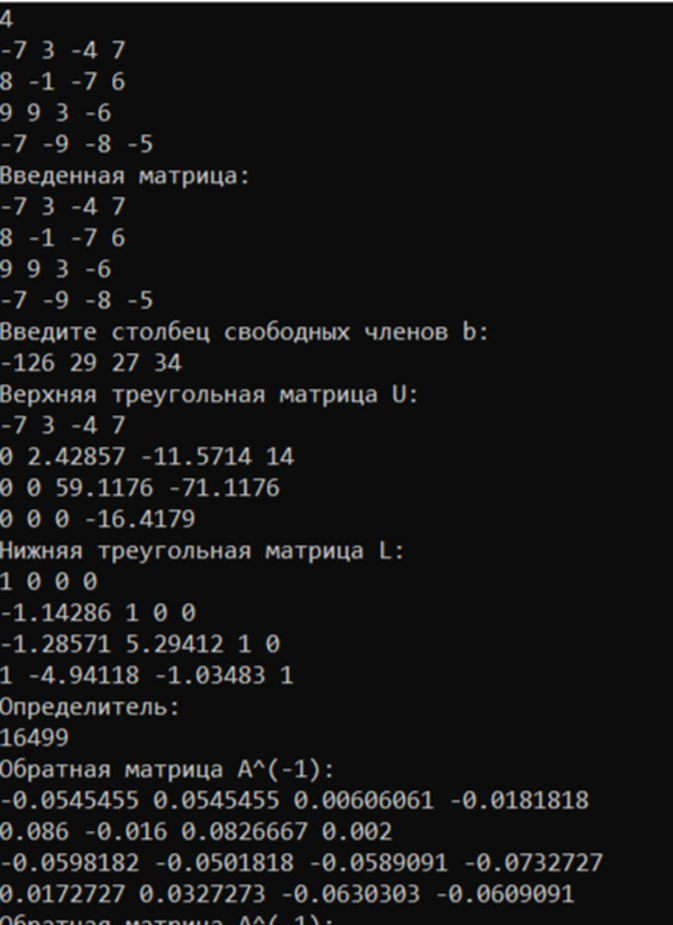
\includegraphics[width=.9\textwidth]{img}
\caption{Вывод программы в консоли}
\end{figure}

% \vfill

% \begin{figure}[h!]
% \centering
% 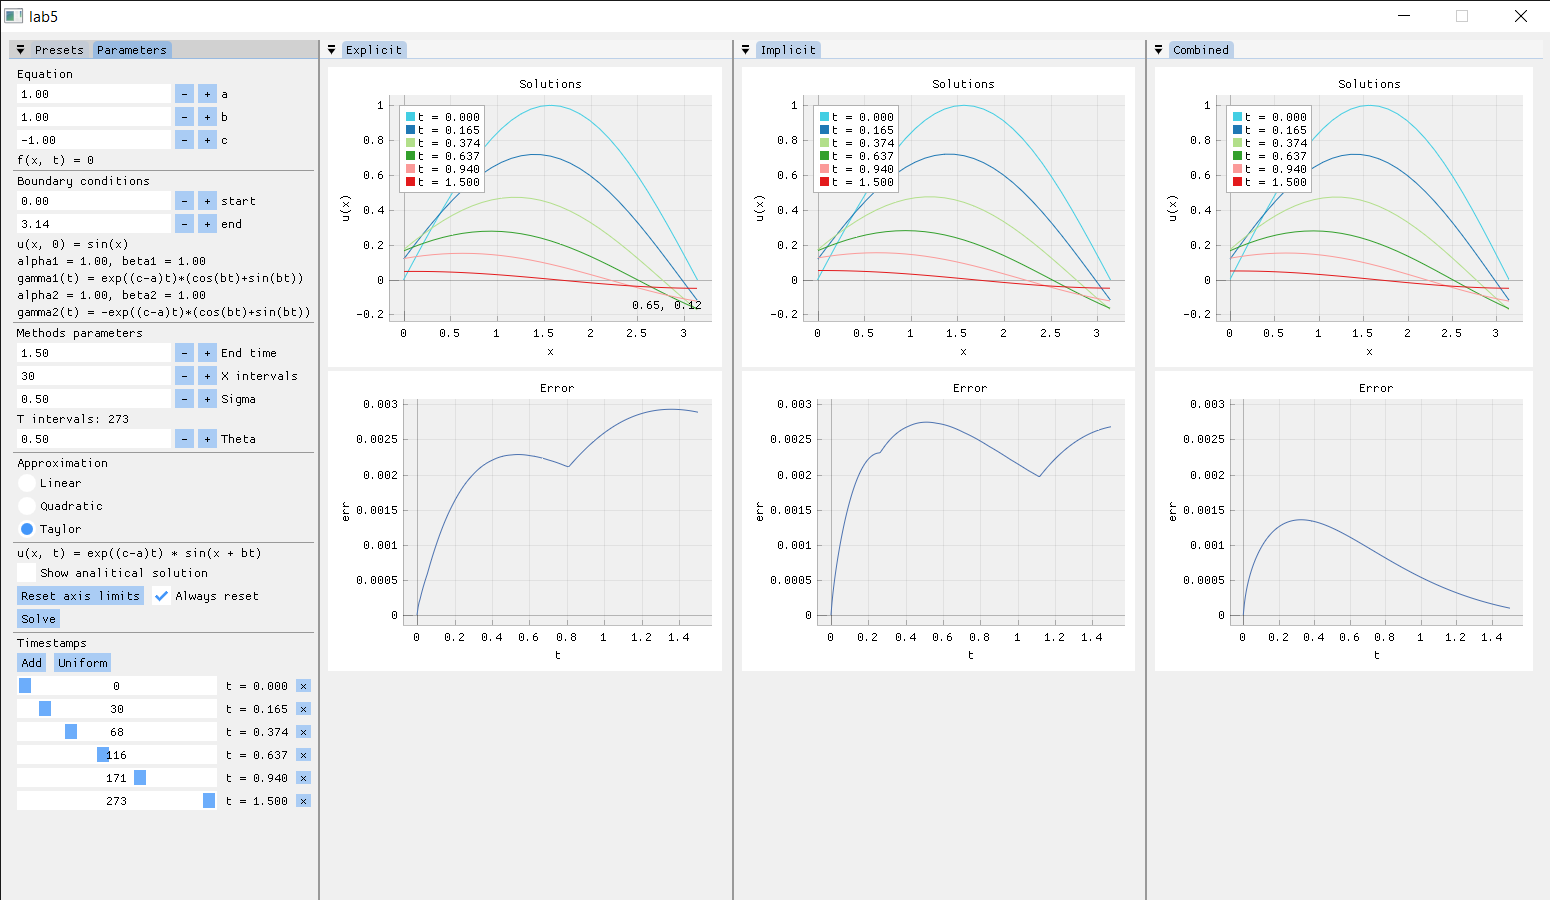
\includegraphics[width=.9\textwidth]{lab5_taylor}
% \caption{Решение с аппроксимацией граничных условий со вторым порядком}
% \end{figure}
\pagebreak

\subsection{Исходный код}
% \lstinputlisting[language=C++]{matrix.cpp}
% \begin{lstlisting}
\lstinputlisting{include/L5.cpp}
% \end{lstlisting}
% \lstinputlisting{matrix.cpp}
% {../../include/matrix.cpp}
% \pagebreak
% \lstinputlisting[title=\texttt{parabolic\_pde.hpp}]{../../include/partial_differential/parabolic_pde.hpp}
% \pagebreak
% 